
\subsection{Solubility Coefficients}

The dissolution behavior of a solute in an aqueous solutions is called its 
solubility. This behavior is limited by the solute's solubility limit, described  
by an equilibrium constant that depends upon temperature, water chemistry, and 
the properties of the element. The equilibrium constant for many reactions are 
known, and can be found in chemical tables.

For solubility limits below a threshold, the dose releases were directly 
proportional to the solubility limit, indicating that the radionuclide 
concentration saturated the groundwater up to the solubility limit near the 
waste form.  For solubility limits above the threshold, however, further 
increase to the limit had no effect on the peak dose. This demonstrates the 
situation in which the solubility limit is so high that even complete 
dissolution of the waste inventory into the pore water is insufficient to reach 
the solubility limit.

In Figures \ref{fig:SolSum}, for example, it is clear that for 
solubility constants lower than a threshold, the relationship between peak 
annual dose and solubility limit is strong.

\begin{figure}[ht]
  \centering
  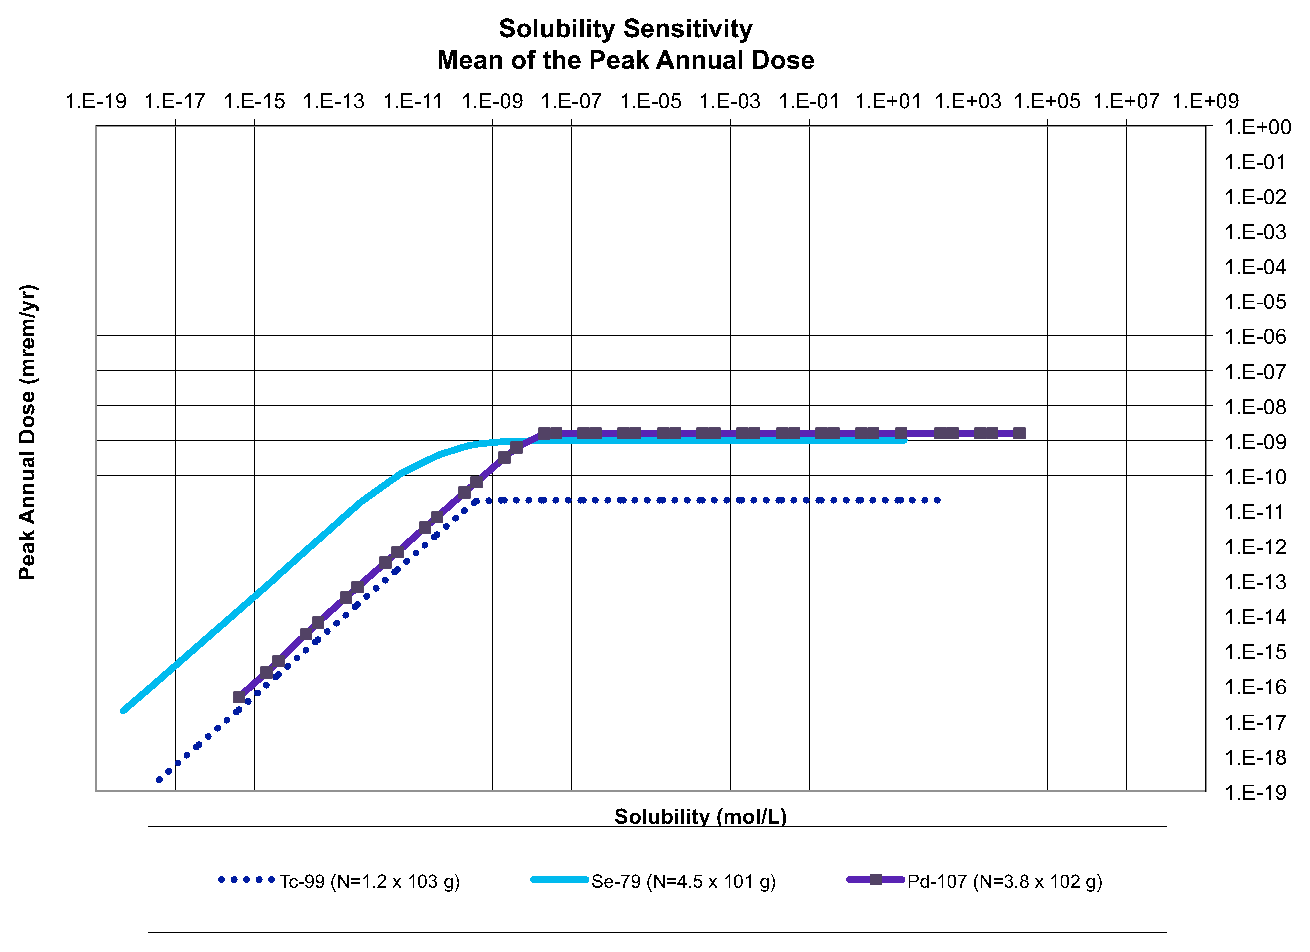
\includegraphics[width=\linewidth]{Solubility_Summary.eps}
  \caption{Solubility limit sensitivity. The peak annual dose due to an 
  inventory, 
  $N$, of each isotope.}
  \label{fig:SolSum}
\end{figure}
